\section{Problema}

% You can reveal the parts of a slide one at a time
% with the \pause command:
\begin{frame}{Problema}
  \begin{itemize}
    \item Edición de imágenes a nivel local. Aplicar cambios a una región de una imagen.
    \item<2-> Planteamiento: 3 Ecuaciones de Poisson usando Cholesky.
    \item<3-> Espacio de trabajo: \textit{RGB}.
  \end{itemize}
\end{frame}

\section{Procedimiento y solución de Poisson}
\begin{frame}{Procedimiento y solución de Poisson}
  \begin{itemize}
    \item Minimizar: \[min_{f}\int \int_{\Omega} \parallel \bigtriangledown f-V\parallel^{2}\] con \[f|\partial_{\Omega}=f^{*}|\partial_{\Omega}\] V es el guidance field.
    \item<2-> \[\bigtriangledown =\left [\frac{\partial }{\partial x},\frac{\partial }{\partial y} \right ]\] Operador de gradiente
    \item<3->
  \end{itemize}
\end{frame}

\begin{frame}{Procedimiento y solución de Poisson}
  \begin{itemize}
    \item Su solución es la única solución a la ecuación: $\Delta f=div V$ con $f|\partial_{\Omega}=f^{*}|\partial_{\Omega}$
    \item<2-> $\Delta=\frac{\partial^2 }{\partial x^2}+\frac{\partial^2 }{\partial y^2}$ es el operador
    Laplaciano.
    \item<3-> $div=\frac{\partial }{\partial x}+\frac{\partial }{\partial y}$ es el operador de divergencia.
    \item<4-> Para nosotros: Resolver 3 ec $Ax=b$, de donde $x=A ^{-1}*b$ o $x=A\setminus b$
    \item<5-> $A$ es la matriz de coeficientes ($NxN$ pixeles a copiar), $b$ el vector solución (\textit{Guidance field})
  \end{itemize}
\end{frame}

\begin{frame}{Procedimiento y solución de Poisson}
  \begin{block}{}
  La matriz $A$ es de la forma
  \begin{figure}[H]
  \centering
  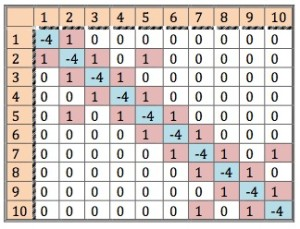
\includegraphics[scale=.4]{./img/kernel}
  \end{figure}
  $b$ es un vector de tres filas (Una por cada canal) y $n$ columnas (Los píxeles de la máscara).
  \end{block}
\end{frame}

\begin{frame}{Procedimiento y solución de Poisson}
  \begin{itemize}
    \item \[ v =\sum_{q\epsilon N_{p}\bigcap \partial\Omega}f^{*}_{q}+\sum_{q\epsilon N_{p}}v_{pq}\]
    \item<2-> El primer termino es la suma de los píxeles vecinos de $p$ que pertenecen a la parte negra de la máscara (No seleccionados), y por tanto son parte de la imagen destino.
    \item<3-> El segundo termino es el gradiente de la imagen. (Se calcula distinto en \textit{normal seamless cloning} y \textit{mixin seamless clonning}  )
  \end{itemize}
\end{frame}

\begin{frame}{Normal Seamless cloning}
  \begin{itemize}
    \item EL gradiente en este caso se obtiene como $v= \bigtriangledown g $, donde $g$ es la imagen fuente.
    \item<2-> Discretizado se traduce en $\forall <p,q>,v_{pq} =g_{p}-g_{q}$. En general buenos resultados si la imagen no presenta transparencias.
  \end{itemize}
\end{frame}

\begin{frame}{Mixin Seamless cloning}
  \begin{itemize}
    \item Mejora el seamless cloning cuando la imagen fuente tiene transparencias.
    \item<2-> Se calcula el guidance Vect tomando el gradiente más fuerte entre la imágen fuente y la imágen de destino.
    \item<3-> $v_{pq}=\left\{\begin{matrix} f^{*}_{p}-f^{*}_{q}$ if $\mid f^{*}_{p}-f^{*}_{q}\mid > \mid g_{p}-g_{q} \mid \\ g_{p}-g_{q} \end{matrix}\right.$
  \end{itemize}
\end{frame}

\begin{frame}{Ejemplos Mixin Seamless}
  \begin{block}{}
  \begin{figure}[H]
  \centering
  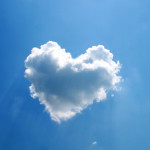
\includegraphics[scale=1]{./img/nube_src}
  \end{figure}
  \end{block}
\end{frame}

\begin{frame}{Ejemplos Mixin Seamless}
  \begin{block}{}
  \begin{figure}[H]
  \centering
  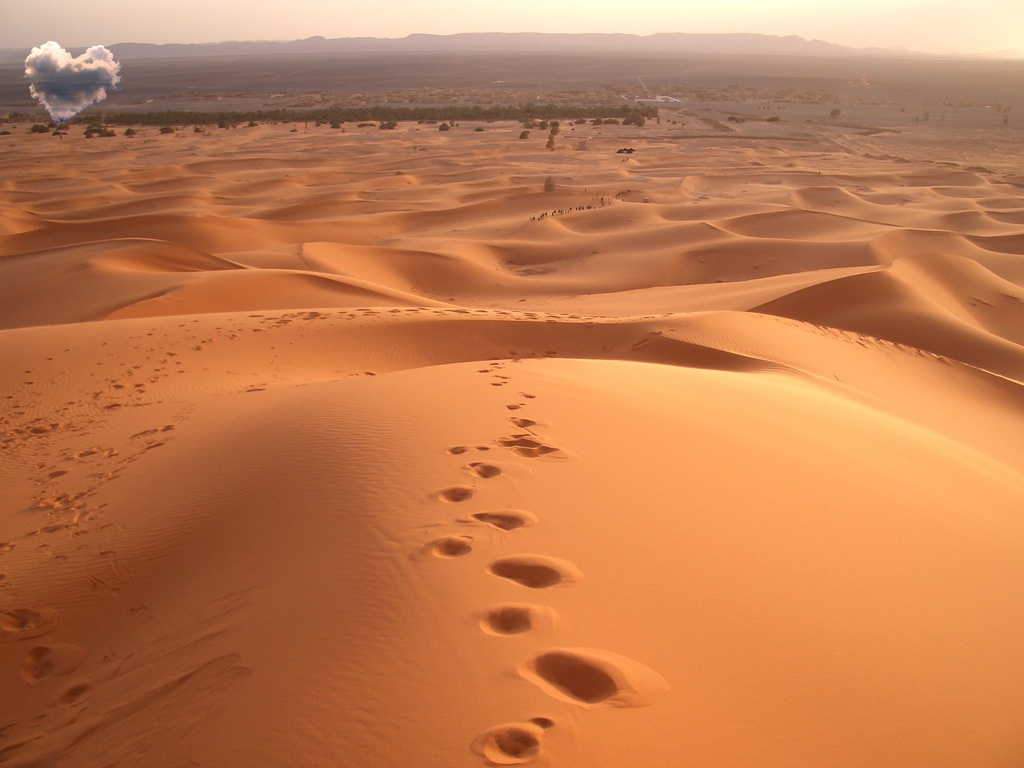
\includegraphics[scale=.5]{./img/desertnube}
  \end{figure}
  \end{block}
\end{frame}

\begin{frame}{Ejemplos Normal Seamless}
  \begin{block}{}
  \begin{figure}[H]
  \centering
  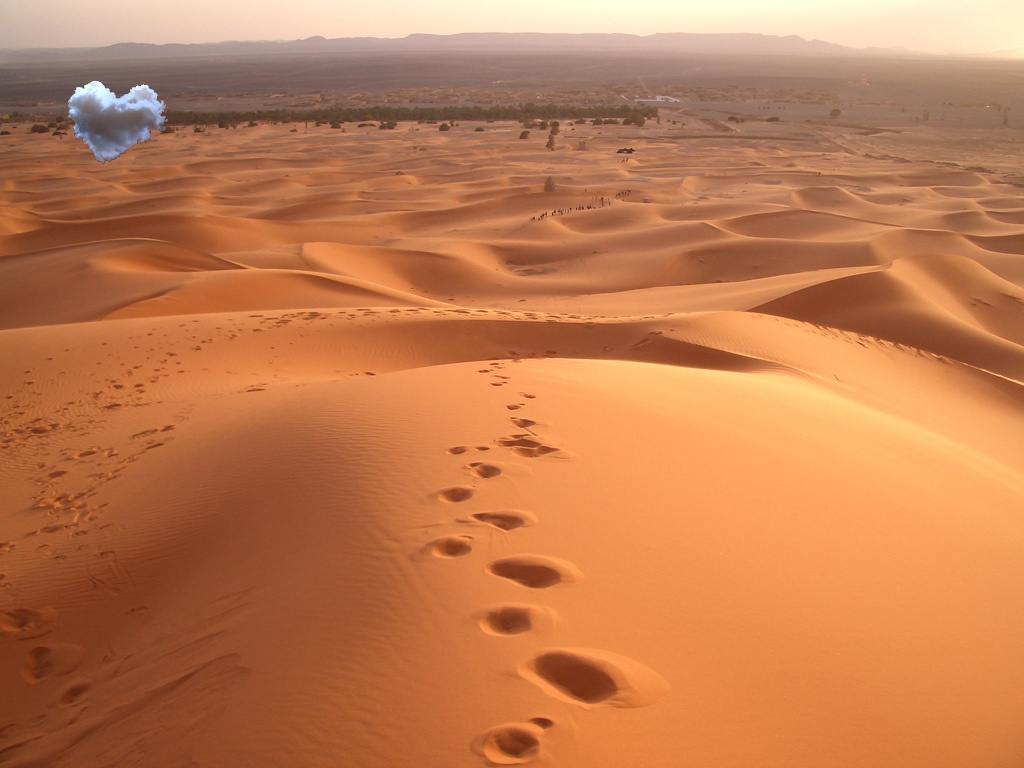
\includegraphics[scale=.5]{./img/normalblue}
  \end{figure}
  \end{block}
\end{frame}

\begin{frame}{Ejemplos mixin Seamless}
  \begin{block}{}
  \begin{figure}[H]
  \centering
  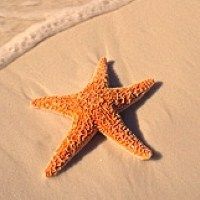
\includegraphics[scale=.5]{./img/estrella_src.jpg}
  \end{figure}
  \end{block}
\end{frame}

\begin{frame}{Ejemplos mixin Seamless}
  \begin{block}{}
  \begin{figure}[H]
  \centering
  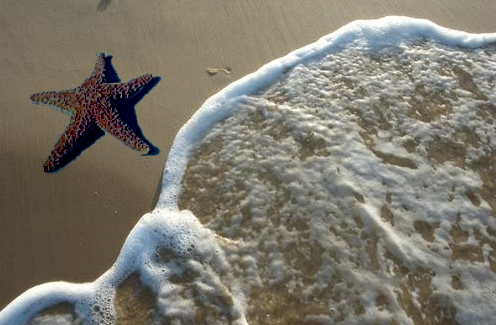
\includegraphics[scale=.5]{./img/mix_seastar}
  \end{figure}
  \end{block}
\end{frame}
